\section{Hybrid Programming} % using MPI+MPI$_{sm}$}

Most HPC systems in use today are clusters of shared memory nodes. The idea of hybrid programming consists of combining parallelization on the node interconnect with parallelization inside of each node. Traditionally, parallelization between nodes is being achieved using a distributed memory programming model such as MPI, while parallelization inside nodes is achieved using a shared memory programming model such as OpenMP, posix threads, or MPI$_{sm}$. 

\medskip

In this section, the performance of hybrid implementations (MPI+OpenMP and MPI+MPI$_{sm}$) of a Jacobi iteration program is evaluated by comparing it to the performance of a traditional (pure) MPI version of the same program. A basic mechanism for hybrid programming involving MPI$_{sm}$ was already presented in in Section \ref{MPISharedMemory}.

\medskip

\subsection*{Jacobi iteration}

The program used to evaluate the hybrid programming model consists a Jacobi iteration solving the 2D-Laplace equation, a common technique to approximate the solution of elliptic PDEs within some allowable tolerance. In this example, a simple stencil calculation is performed, where each point in a 2D grid calculates its new value as the mean of its neighbors' old values, as illustrated in Figure \ref{fig:LaplacePureMPI}. In general the calculation continues until either the maximum change in the value between two iterations drops below some established tolerance or a maximum number of iterations is reached.

\medskip

\begin{figure} [h!]
\centering
\captionsetup{justification=centering, singlelinecheck=false}
\begin{lstlisting}[style=CStyle]
double laplace(double *restrict tNew, double *restrict tOld, int sRow, int eRow)
{
  const int nRows = eRow-sRow + 1;
  double dt=0.0;   // reset largest temperature change
  for(int r = COL2; r <=(nRows*COL2) ; r+=COL2) {
    for(int c = 1; c <= COLUMNS; ++c) {
      tNew[r+c] =  0.25*(tOld[r+c+COL2] + tOld[r+c-COL2] + tOld[r+c+1] + tOld[r+c-1]);
      dt = fabs( tNew[r+c] - tOld[r+c] ) > dt ?  fabs( tNew[r+c] - tOld[r+c] ) : dt;
    } // end for //
  } // end for //
  return dt;
} // end of laplace() //
\end{lstlisting}    
\caption{Two-dimensional stencil for Laplace equation.}
\label{fig:LaplacePureMPI}
\end{figure}


\medskip

Figure \ref{fig:JacobiMPI} presents the core of the \emph{pure} MPI implementation. Lines 3 to 5 contains a iteration counter, the call to the laplace function (Figure \ref{fig:LaplacePureMPI}) and a reduction to determine the larger change in the value of the current iteration. Lines 7 to 21 perform the hallo exchange of the latest values obtained after calling the laplace function and lines 22 to 23 perform pointer swaps before determining, in line 25, if a new iteration is needed. The MPI+OpenMP implementation is essentially the same; the only required change is the addition of an OpenMP work sharing pragma before calling the laplace function.

\medskip

Figure \ref{fig:JacobiMPI+MPI} presents the core of the MPI+MPI$_{sm}$ implementation. The main difference with respect to Figure \ref{fig:JacobiMPI} happen inside the two \emph{\textbf{if}} statements located between lines 7 to 13 and 15 to 21 of Figure \ref{fig:JacobiMPI}. In the MPI+MPI$_{sm}$ implementation these \emph{\textbf{if}} statements now contain a nested \emph{\textbf{if-else}} statement used to determine (using the the \emph{\textbf{localRank}} array) if a given rank belong to the current node, in which case a direct copy of the hollow is done using the memcpy() function, or not.  See the subsection \emph{\textbf{Pseudo Code for hybrid programming}} in Section \ref{MPISharedMemory} for a more detailed explanation describing the use of the \emph{\textbf{localRank}} array.

\begin{comment}

Figure \ref{fig:JacobiMPI+MPI}  

Notice also the use of the the \emph{\textbf{localRank}} array in the nested \textbf{if-else} statement.

Notice in Figure \ref{fig:JacobiMPI+MPI} the use of 

to determine if a given rank belong to the current node, in which case a direct copy of the hollow is done using the memcpy() function, or not. 
\end{comment}



\begin{figure} [t!]
\centering
\captionsetup{justification=centering, singlelinecheck=false}
\begin{lstlisting}[style=CStyle]
// do until error is minimal or until max steps
do {
  ++iteration;
  dt = laplace(Temperature,Temperature_last, sRow,eRow);
  MPI_Allreduce(MPI_IN_PLACE,&dt, 1,MPI_DOUBLE,MPI_MAX,MPI_COMM_WORLD);

  if (myWorldRank < worldSize-1) { 
    MPI_Irecv(&Temperature[(nRows-1)*COL2],COL2,MPI_DOUBLE,
               myWorldRank+1,200,MPI_COMM_WORLD,&request[0]);
    MPI_Isend(&Temperature[(nRows-2)*COL2],COL2,MPI_DOUBLE,
              myWorldRank+1,100,MPI_COMM_WORLD,&request[1]);
    MPI_Waitall(2,request, status);
  } // end if //  

  if (myWorldRank > 0)  {
    MPI_Irecv(&Temperature[0]   ,COL2,MPI_DOUBLE,
               myWorldRank-1,100,MPI_COMM_WORLD,&request[0]);
    MPI_Isend(&Temperature[COL2],COL2,MPI_DOUBLE,
               myWorldRank-1,200,MPI_COMM_WORLD,&request[1]);
    MPI_Waitall(2,request, status);
  } // end if //   
  temp = Temperature_last;
  Temperature_last=Temperature;
  Temperature=temp;           
} while (dt > MAX_TEMP_ERROR && iteration < max_iterations) ; // end do-while //
\end{lstlisting}    
\caption{Jacobi iteration - Pure MPI implementation.}
\label{fig:JacobiMPI}
\end{figure}




\medskip

\begin{figure} [h!]
\centering
\captionsetup{justification=centering, singlelinecheck=false}
\begin{lstlisting}[style=CStyle]
// do until error is minimal or until max steps
do {
  ++iteration;
  dt = laplace(Temperature,Temperature_last,nRows-2);
  MPI_Allreduce(MPI_IN_PLACE,&dt, 1,MPI_DOUBLE,MPI_MAX,MPI_COMM_WORLD);

  if (myWorldRank < worldSize-1) { 
    if (localRank[myWorldRank+1] != MPI_UNDEFINED) {
      memcpy(&Temperature[(nRows)*COL2],&Temperature[(nRows-2)*COL2], COL2*sizeof(double));
    } else {
      MPI_Irecv(&Temperature[(nRows-1)*COL2],COL2,MPI_DOUBLE,
                 myWorldRank+1,200,MPI_COMM_WORLD,&request[0]);
      MPI_Isend(&Temperature[(nRows-2)*COL2],COL2,MPI_DOUBLE,
                 myWorldRank+1,100,MPI_COMM_WORLD,&request[1]);
      MPI_Waitall(2,request, status);
    } // end if //  
  } // end if //  

  if (myWorldRank > 0)  {
    if (localRank[myWorldRank-1] != MPI_UNDEFINED) {
      memcpy(&Temperature[-COL2],&Temperature[COL2], COL2*sizeof(double));
    } else {
      MPI_Irecv(&Temperature[0]   ,COL2,MPI_DOUBLE,
                 myWorldRank-1,100,MPI_COMM_WORLD,&request[0]);
      MPI_Isend(&Temperature[COL2],COL2,MPI_DOUBLE,
                 myWorldRank-1,200,MPI_COMM_WORLD,&request[1]);
      MPI_Waitall(2,request, status);
    } // end if //
  } // end if //
  temp = Temperature_last;
  Temperature_last=Temperature;
  Temperature=temp;        
} while (dt > MAX_TEMP_ERROR && iteration < max_iterations) ; // end do-while //
\end{lstlisting}    
\caption{Jacobi iteration - MPI+MPI$_{sm}$ implementation.}
\label{fig:JacobiMPI+MPI}
\end{figure}


\subsubsection*{Single Node Results}

The problem at hand consist in solving a 4096 X 4096 grid. In general, the domain is divided by rows. While the pure MPI and the hybrid MPI+MPI$_{sm}$ programs divide the domain in as many parts as processes (ranks) involved in the solution, the hybrid MPI+OpenMP program uses a single MPI process and multiple OpenMP threads to solve the problem.

\medskip

Figure \ref{fig:HybridSingleNode} shows results comparing the performance (time) of two hybrid implementations as well as the pure MPI case running in a single node (\textbf{koelsch}). This results correspond to the GNU compiler and openmpi. Results from the others compilers (Intel and Pgi) were similar. As usual, the left plot (\ref{fig:HybridSingleNodeComparison}) shows actual execution time while the right plot (\ref{fig:HybridSingleNodeRatioComparison}) presents the ratio between the time taken by the pure MPI program to each of the hybrid ones. From Figure \ref{fig:HybridSingleNodeComparison} it is clear that the execution time of the three programs is similar. However, Figure \ref{fig:HybridSingleNodeRatioComparison} allows to see that, in general, the performance of the hybrid programs exceed for a small margin that of the non-hybrid one.

\medskip


\begin{figure} [h!]
    \centering
    \captionsetup{justification=centering, singlelinecheck=false}
    \begin{subfigure}{.6\textwidth}
      \centering
      \hspace*{-1.5cm} 
      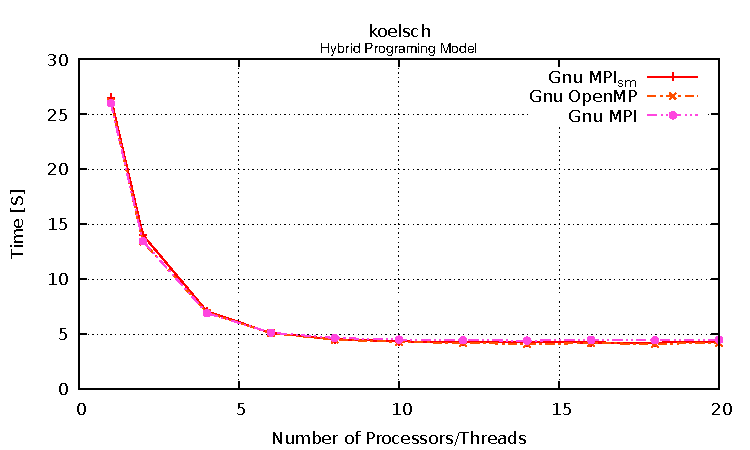
\includegraphics[page=1,width=0.95\linewidth]{Plots/HybridProgramming/koelsch_Gnu.pdf}
      \caption[]{Estimated time.}
      \label{fig:HybridSingleNodeComparison}
    \end{subfigure}%
    \begin{subfigure}{.6\textwidth}
      \centering
      \hspace*{-1.5cm} 
      \includegraphics[page=2,width=0.95\linewidth]{Plots/HybridProgramming/koelsch_Gnu.pdf}
      \caption{Pure MPI to Hybrids Ratio.}
      \label{fig:HybridSingleNodeRatioComparison}
    \end{subfigure}%
\caption{Pure MPI to Hybrids comparison in a single node.}
\label{fig:HybridSingleNode}
\end{figure}



\begin{figure}[h!]
    \centering
    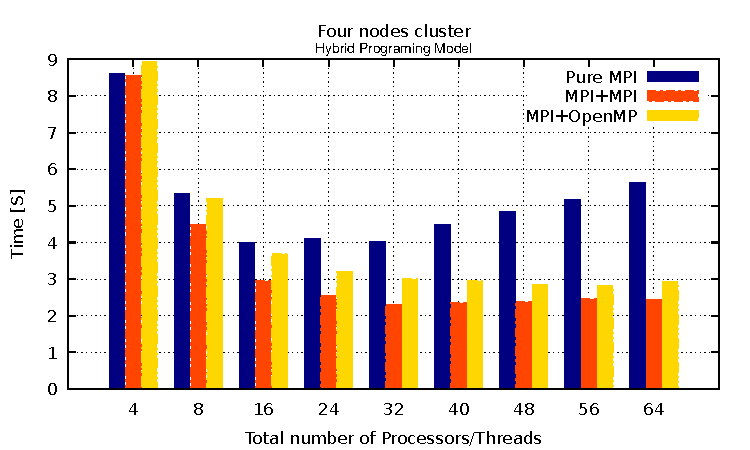
\includegraphics[width=100mm]{Plots/HybridProgramming/cluster.pdf}
    \caption{Jacobi iteration solving the 2D-Laplace equation in a four-node cluster.}
    \label{fig:HybridCluster}
\end{figure}



\begin{comment}
  \begin{figure}[h!]
      \centering
      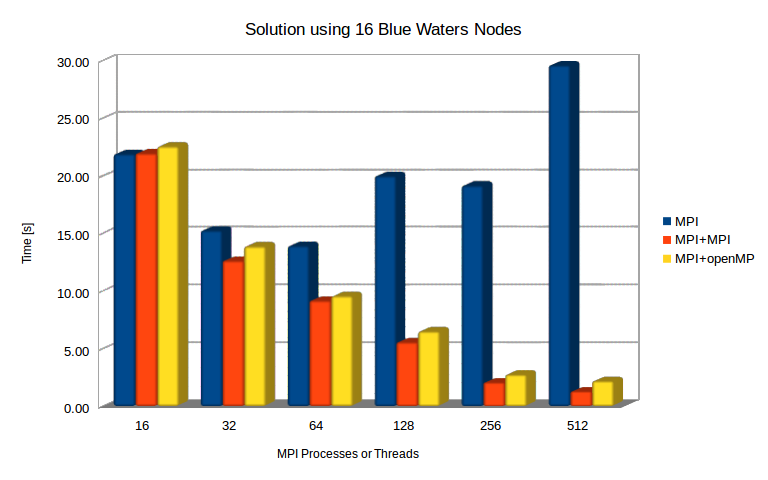
\includegraphics[width=100mm]{Plots/HybridProgramming/bw2-16.png}
      \caption{Jacobi iteration solving the 2D-Laplace equation.}
      \label{fig:Figure5}
  \end{figure}
\end{comment}


\subsubsection*{Four Node Cluster}

The potential benefits of MPI+ hybrid programming can be better appreciated by running the programs in a cluster. Figure \ref{fig:HybridCluster} show results obtained from running the programs in a four-nodes cluster. The horizontal axis shows the total number of processors/threads used in each run. The number of processors/threads used per node was the same, therefore, the total number of processors/thread is always a factor of four. For example, 8 processors/threads per node were used for the case of 32 total processors/threads. %In other words, the number of processors/threads used in each node is equal to the total number of processors/threads divided by four.

\medskip

Notice that in this example, the volume of inter-node communication, which is done using conventional send/receive MPI functions, is constant and independent of number of processors/threads per node utilized. Its impact on performance is the same for all the programs, pure and hybrids.

Contrastively, inside a node, the number of processors/threads per node produce a proportional growing of the number of conventional send/receive calls in the pure MPI case, while no extra conventional send/receive calls are required for the hybrid versions since all the extra communication is done via shared memory.

volve a leer y aprobar....

%do have a bigger impact , because it . 

%On the other hand, the impact on the hybrid versions is smaller because this intra-node communication is done via shared memory.

\medskip

%For the pure MPI program, as more processes are used per node the amount of inter-node communication using conventional send/receive mpi functions grows. 

%For the MPI+MPI$_{sm}$ hybrid version  as more processes are used per node  

\medskip

Figure \ref{fig:HybridCluster} allows to make several comments. 


\begin{itemize} 
\item In the case of one processor/thread per node (four total processors/threads) the performance of the pure MPI program and of the two hybrids are similar. This result is in accordance with what can be observed in Figure \ref{fig:HybridSingleNode} for one processor/thread.

\item Sec

\item Sec

\item Sect



\end{itemize}



The hybrid versions of the program sub-divide the grid, by rows, in 16 parts, handling each of this parts in a separate node. Therefore they have only communication among the nodes (inter-node communication). Inside each node the hybrid versions use an increasing number of threads (OpenMP) or processes (MPI$_{sm}$) to handle their part of the problem without any communication involved.

On the other hand, the MPI version brake the gird in as many parts as total MPI rank are used in the solution; for example for the 256 total ranks, there are 256 MPI communication boundaries to deal with. Although most of the communication corresponds to intra-node boundaries, those intra-node communication are handled by the send/receive family of MPI functions. Additionally, the MPI version still have to deal with 16 communications corresponds to the original 16 inter-node boundaries.


\subsection*{Be aware of binding}

Comentar sobre experiencia con gcc+openMPI(3.1.0)

%Additionally it shows that the MPI+MPI$_{sm}$ approach can outperform the MPI+OpenMP version.




\begin{comment}

\subsection*{Hybrid programming in MPI}
While in the hybrid programming combining MPI and OpenMP (MPI+OpenMP), it is usual to have several OpenMP threads inside a node and (frequently) one MPI processes per node, in the MPI+MPI$_{sm}$ hybrid programming everything is an MPI process. Therefore, the MPI+MPI$_{sm}$ hybrid programming requires a mechanism to distinguish between processes that exist inside a node and those belonging to different node. Therefore, this section start with a brief description of MPI function and datatypes that can be used to accomplish this goal. The pseudo code bellow can help to describe the important steps in this process. 

\medskip
Two variables of type MPI\_Group, one for the whole set of ranks and one for the ranks belonging to a node are needed. This is shown in line 7 of the pseudo code. These variables are used to define global and shared group communicators using the MPI\_Comm\_group() function as shown in lines 8 an 9. 


\begin{lstlisting}[style=CStyle]
#include <stdlib.h>
#include <stdio.h>

int main(int argc, char *argv[]) 
{
    .
    MPI_Group sharedGroup,worldGroup;
    MPI_Comm_group(MPI_COMM_WORLD, &worldGroup);
    MPI_Comm_group(sm_comm, &sharedGroup);
    .
    int *partners, *map;
    partners = (int *)malloc( worldSize * sizeof(int) );
    map      = (int *)malloc( worldSize * sizeof(int) );
    .
    MPI_Group_translate_ranks(worldGroup, worldSize, partners, sharedGroup, map);
    .
    if (map[myWorldRank+1] != MPI_UNDEFINED) {
        memcpy(&Temperature[(nRows)*COL2],&Temperature[(nRows-2)*COL2],...);
    } else {
        MPI_Irecv(&Temperature[(nRows-1)*COL2],....);
        MPI_Isend(&Temperature[(nRows-2)*COL2],....);
        MPI_Waitall(2,request, status);
    } // end if //  
    return 0;
} // end main() // 
\end{lstlisting}


Also needed are a couple of integer pointers which need to be allocated to the size of the MPI\_WORLD\_COMM (the total number of MPI processes used for the program), lines 11 to 13. These pointers are used to map global rank numbers to shared rank numbers using the function MPI\_Group\_translate\_ranks(), shown in line 15. The \emph{map} pointer is of special interest. Each element of this pointer represent each one of the MPI processes used by the program. After the MPI\_Group\_translate\_ranks() is called, all the elements of the \emph{map} pointer, except those corresponding to processors belonging to a given node are set to an undefined state (MPI\_UNDEFINED). This can be used to determine the type of communication a given process can have with another process depending on the location (inter-node vs intra-node) of that process, as shown in lines 17 to 23.

\end{comment}

